% app5.tex
\chapter{Multiphonic Fingering Chart}\label{app:Multiphonic Fingering Chart}
Adapted from Fallowfield's website CelloMap, which as of time of publication, is not currently online.\autocite[http://www.cellomap.com/index/the-string/multiphonics-and-other-multiple-sounds/fingeringcharts.html]{fallowfieldCelloMap}
This shows the two nodes where multiphonics can be produced, and the resultant pitch for both of them.
It includes the tuning in cents, and the partial ratios (i.e.\ 7+13+6). 
It should be noted that this is a fingering reference tool, and not to be used for notation (see \autoref{sec:notation-multiphonics} for notation of multiphonics.)
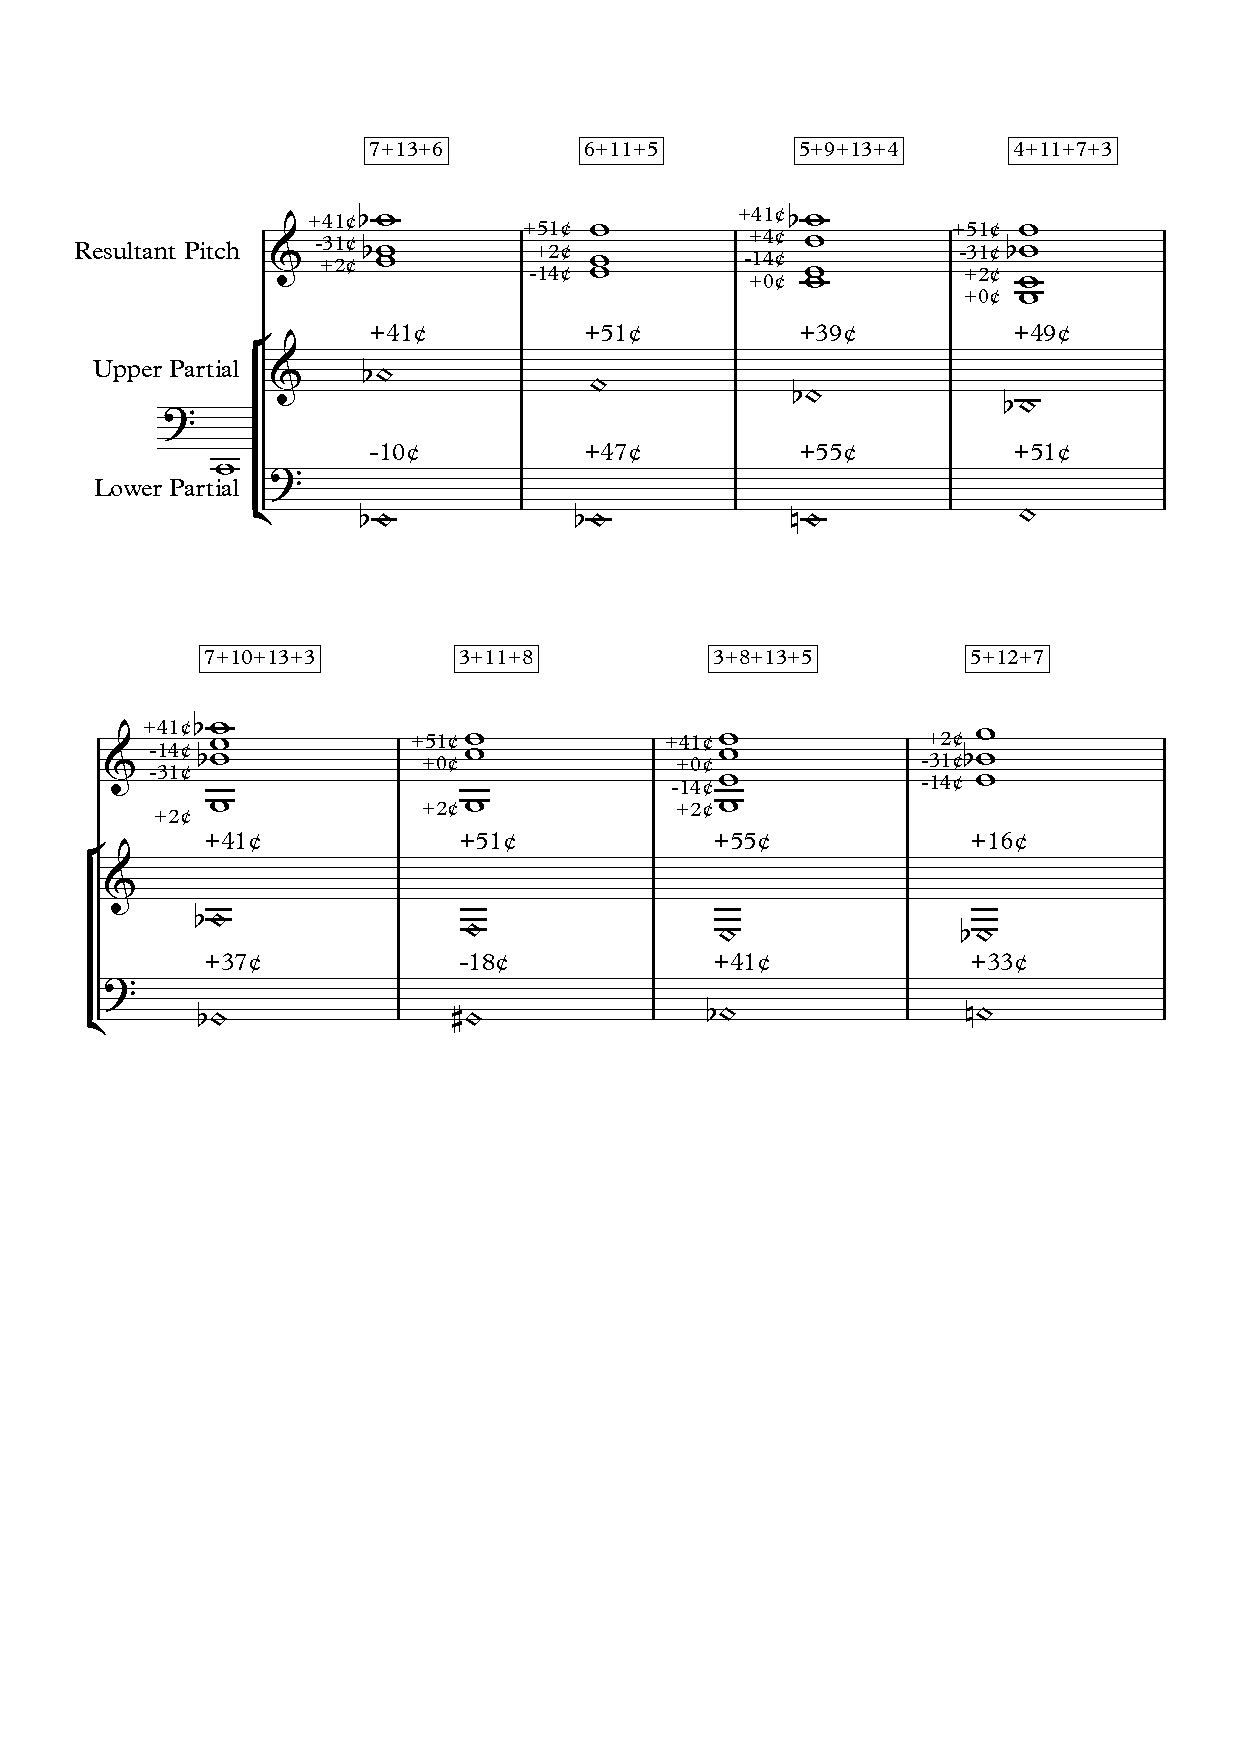
\includepdf[pages=-,pagecommand={}]{resources/multiphonicFingeringChart.pdf}